\documentclass[xcolor=table,handout]{beamer}
\setbeamertemplate{navigation symbols}{}

\usepackage{pgfpages}
\usepackage{adjustbox}
\setbeameroption{show notes}
\setbeameroption{show notes on second screen=right}

\usepackage{booktabs}
\usepackage{beamerthemeshadow}
\setbeamertemplate{caption}[numbered]
\setbeamerfont{caption}{size=\tiny}

\begin{document}

\title{Journal Club Presentation: Ocean Color}  
\author[K. Bellock, L. Chen, D. Durrance, A. Yen, H. Perez]{Kenneth Bellock, Leshi Chen, Danielle Durrance, Andrew Yen, Hack Perez}
\titlegraphic{%
    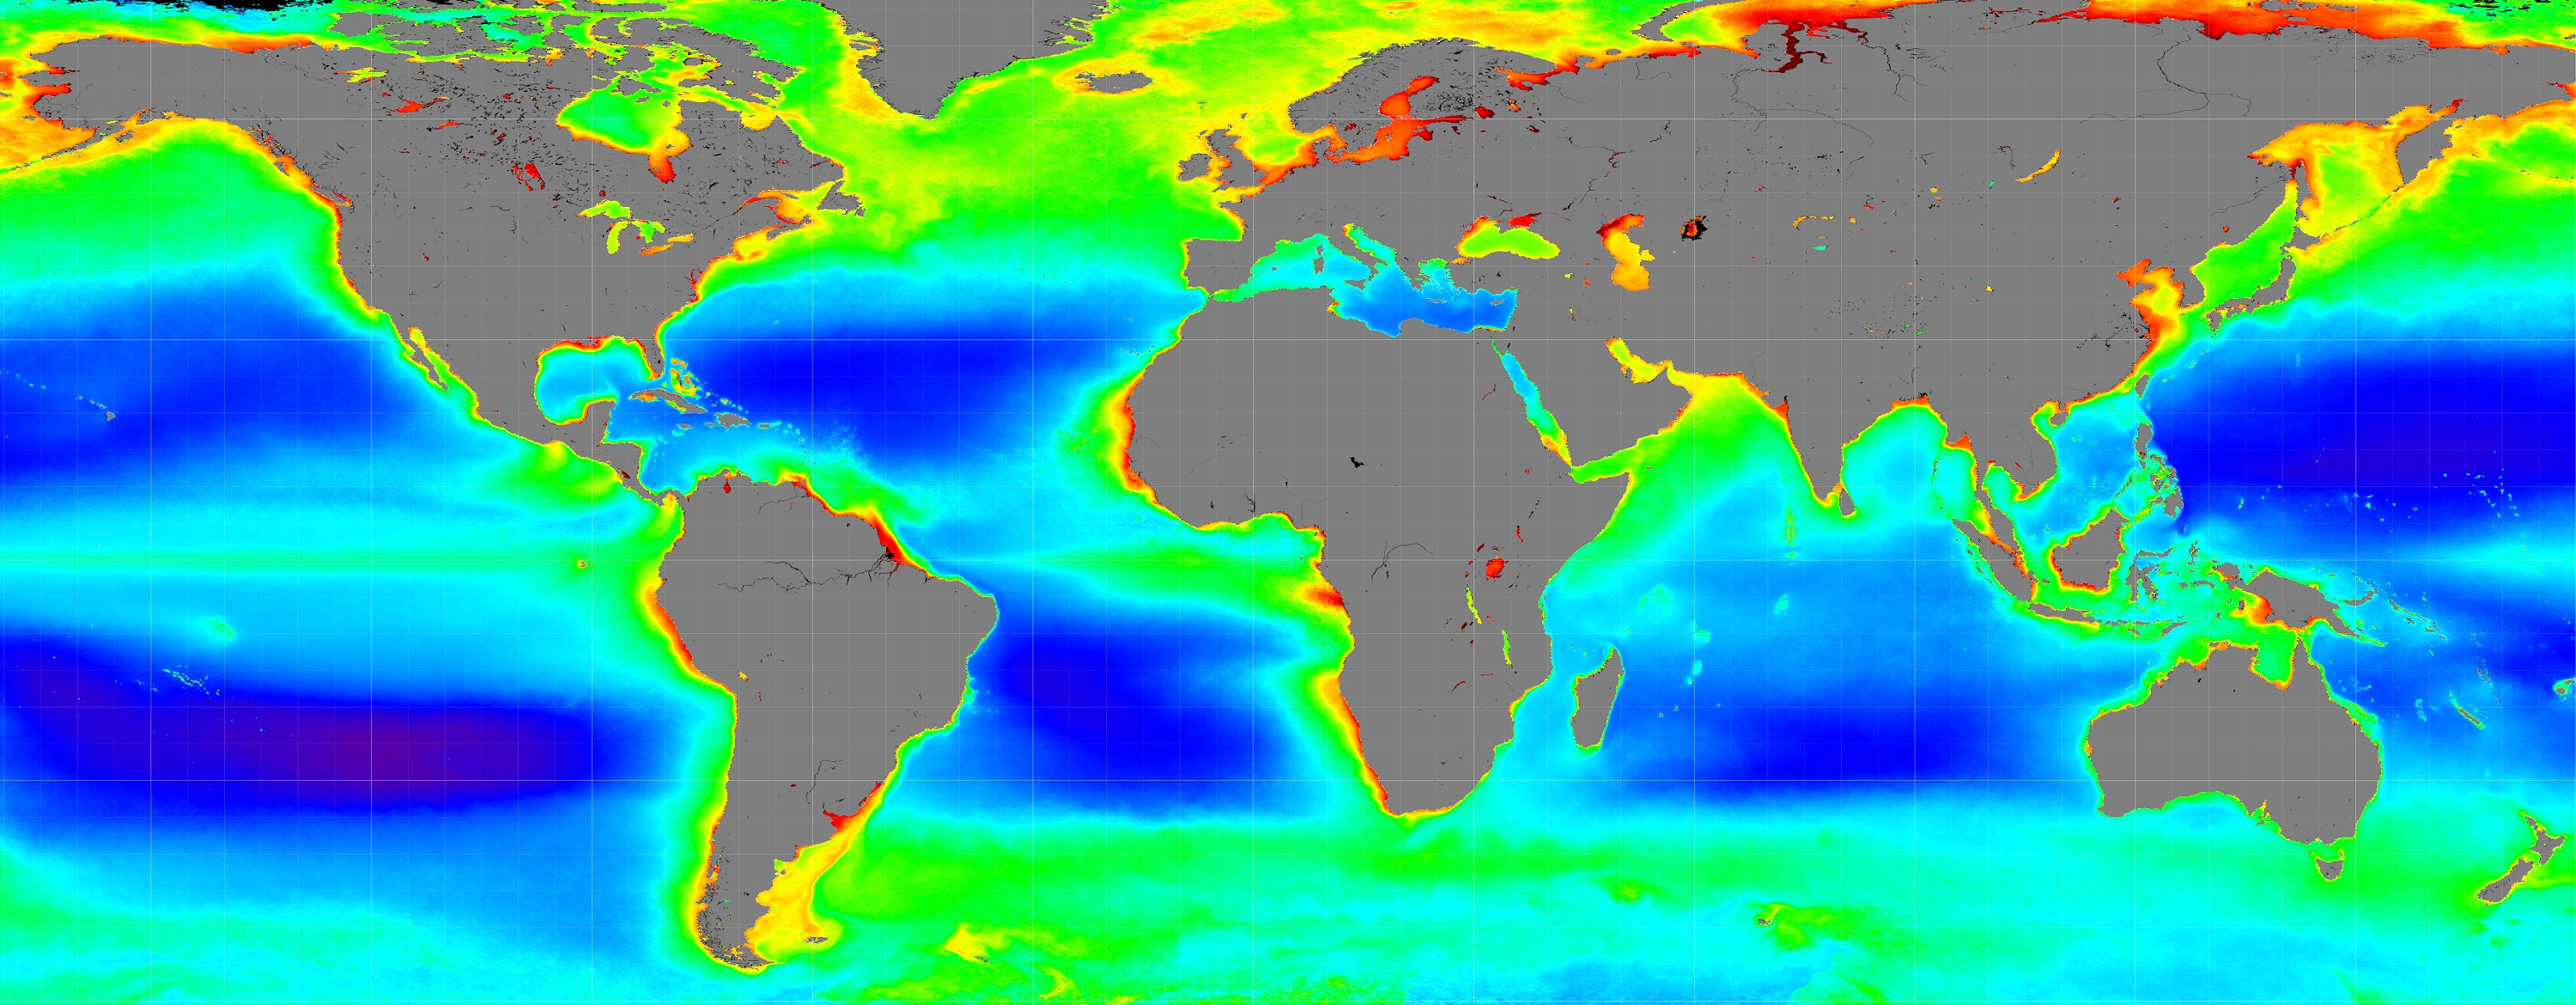
\includegraphics[height=.37\textheight]{15_037}

    \tiny \textbf{Source:} \url{https://www.nasa.gov/press/2015/march/new-nasa-mission-to-study-ocean-color-airborne-particles-and-clouds}
}
\date{\vspace*{-2.5em}\par April 4, 2018} 

\section{Introduction}

\begin{frame}
  \titlepage{}
  \note{Assumptions:}
  \note[item]{TODO:\@ List assumptions.}
\end{frame}

\begin{frame}\frametitle{Table of contents}
  \tableofcontents{}
  \note[item]{A road map is a great thing to have.}
  \note[item]{A joke or reference to current events in common culture would be great here if the audience appears receptive.}
\end{frame} 

\begin{frame}\frametitle{Introduction} 

  \note[item]{TODO:\@ Write Introduction}
\end{frame}


\section{Article Summaries}

\begin{frame}\frametitle{Biospheric Primary Production During an ENSO Transition} 

\begin{description}
    \item[Authors] Michael J. Behrenfield, James T. Randerson, Charles R. McClain, Gene C. Feldman, Sietse O. Los, Compton J. Tucker, Paul G. Falkowski, Christopher B. Field, Robert Frouin, Wayne E. Esaias, Dorota D. Kolber, Nathan H. Pollack
    \item[Objectives] TODO: Include objectives.
    \item[Methods] TODO: Include methods.
    \item[Findings] TODO: Include findings.
\end{description}

  \note[item]{Include notes and talking points here.}
  \note[item]{There can be more than one note.}
\end{frame}

\begin{frame}\frametitle{Biospheric Primary Production During an ENSO Transition} 
    \begin{center}
        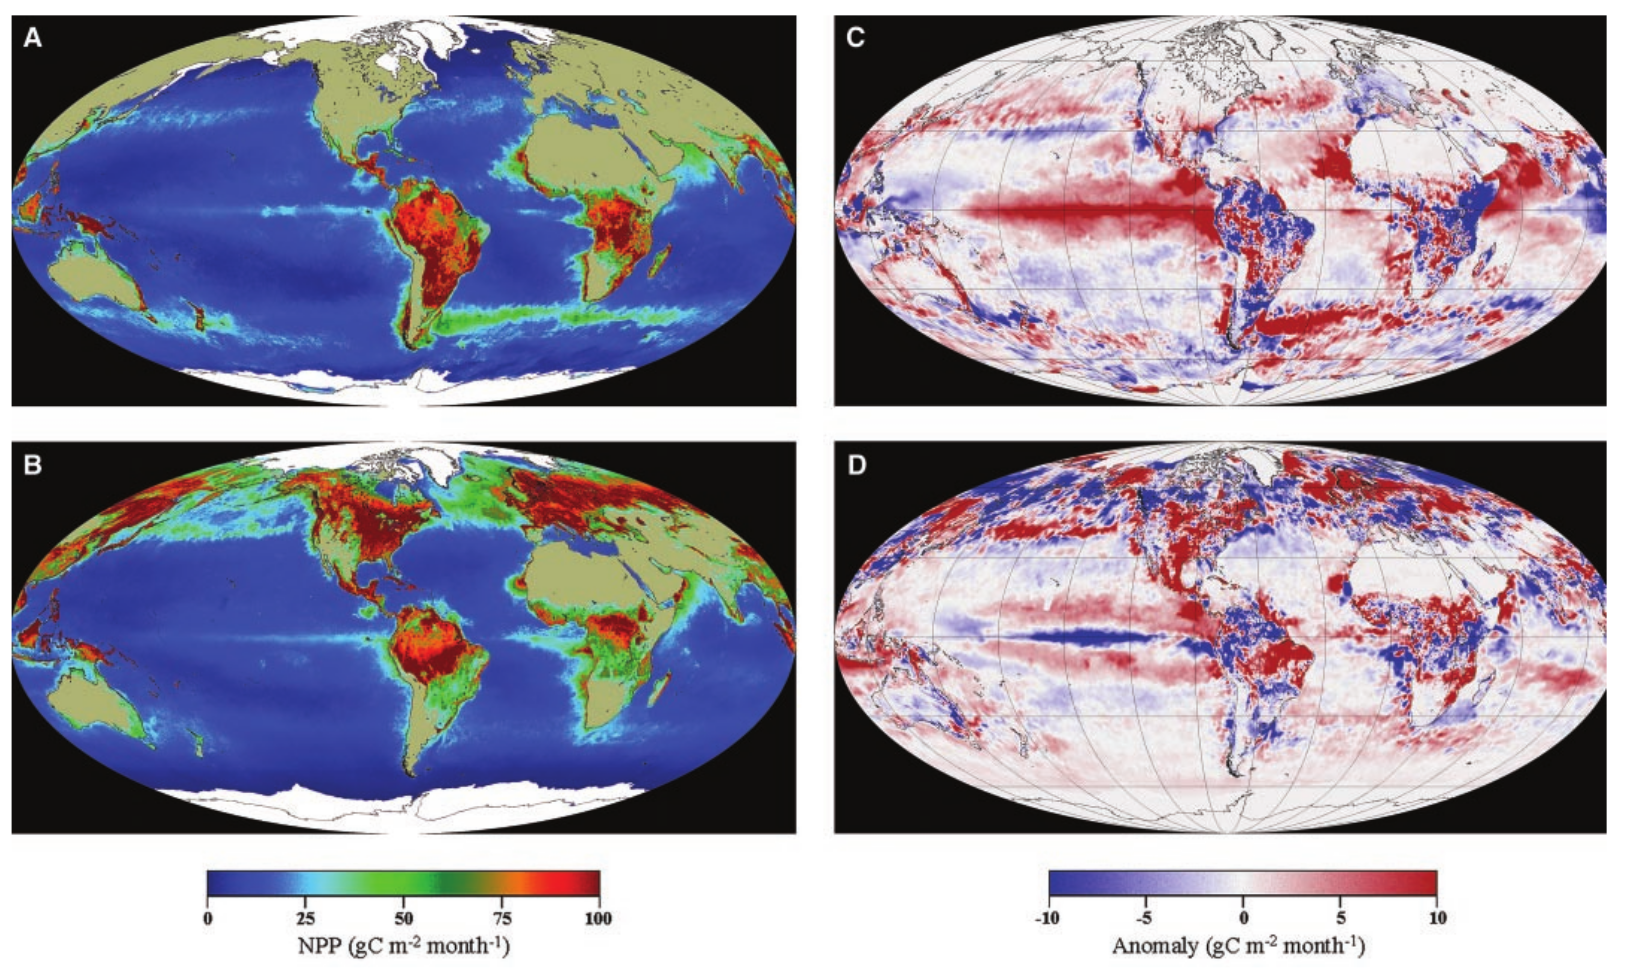
\includegraphics[width=\textwidth,height=0.8\textheight,keepaspectratio]{npp}
    \end{center}
  \note[item]{Pretty picture}
\end{frame}

\begin{frame}\frametitle{Performance of the MODIS semi-analytical ocean color algorithm for chlorophyll-a} 
\begin{description}
    \item[Authors] K.L. Carder, F.R. Chen, J.P. Cannizzaro, J.W. Campbell, B.G. Mitchell
    \item[Objectives] TODO: Include objectives.
    \item[Methods] TODO: Include methods.
    \item[Findings] TODO: Include findings.
\end{description}

  \note[item]{Include notes and talking points here.}
  \note[item]{There can be more than one note.}
\end{frame}

\begin{frame}\frametitle{Performance of the MODIS semi-analytical ocean color algorithm for chlorophyll-a} 

  \note[item]{TODO:\@ Include a pretty picture.}
\end{frame}

\begin{frame}\frametitle{Decadal changes in global ocean chlorophyll} 
\begin{description}
    \item[Authors] Watson W. Gregg, Margarita E. Conkright
    \item[Objectives] TODO: Include objectives.
    \item[Methods] TODO: Include methods.
    \item[Findings] TODO: Include findings.
\end{description}

  \note[item]{Include notes and talking points here.}
  \note[item]{There can be more than one note.}
\end{frame}

\begin{frame}\frametitle{Decadal changes in global ocean chlorophyll} 

  \note[item]{TODO:\@ Include a pretty picture.}
\end{frame}

\begin{frame}\frametitle{Corrections to the Calibration of MODIS Aqua Ocean Color Bands Derived From SeaWiFS Data} 
\begin{description}
    \item[Authors] Gerhard Meister, Bryan A. Franz, Ewa J. Kwiatkowska, Charles R. McClain
    \item[Objectives] TODO: Include objectives.
    \item[Methods] TODO: Include methods.
    \item[Findings] TODO: Include findings.
\end{description}

  \note[item]{Include notes and talking points here.}
  \note[item]{There can be more than one note.}
\end{frame}

\begin{frame}\frametitle{Corrections to the Calibration of MODIS Aqua Ocean Color Bands Derived From SeaWiFS Data} 

  \note[item]{TODO:\@ Include a pretty picture.}
\end{frame}


\section{Summary and Conclusion}

\begin{frame}\frametitle{Summary} 

  \note[item]{TODO:\@ Write Summary}
\end{frame}

\begin{frame}\frametitle{Conclusion} 

  \note[item]{TODO:\@ Write Conclusion}
\end{frame}


\end{document}
